\documentclass{article}
\usepackage[utf8]{inputenc}
\documentclass[12pt]{article}
%\usepackage[left=3cm, right=2.5cm, top=2.5cm, bottom=2.5cm]{geometry}e}
\usepackage[utf8]{inputenc}
\usepackage[spanish,english]{babel}
\usepackage{apacite}
\usepackage[round]{natbib}
\usepackage{hyperref}
\usepackage{float}
\usepackage{svg}
\usepackage[margin = 1in, top=2cm]{geometry}% Margins
\setlength{\parindent}{2em}
\setlength{\parskip}{0.2em}
\usepackage{setspace} % Setting the spacing between lines
\usepackage{amsthm, amsmath, amsfonts, mathtools, amssymb, bm} % Math packages 
\usepackage{svg}
\usepackage{graphicx}
\usepackage{pgfplots}
\usepackage{epstopdf}
%\usepackage{subfig} % Manipulation and reference of small or sub figures and tables
\usepackage{hyperref} % To create hyperlinks within the document
\spacing{1.15}
\usepackage{appendix}
\usepackage{xcolor}
\usepackage{cancel}
\usepackage{enumerate}
\usepackage{subcaption}
\usepackage[shortlabels]{enumitem}


\usepackage[round]{natbib}
%\bibliographystyle{plainnat}
\bibliographystyle{apacite}


\newtheorem{defin}{Definition.}
\newtheorem{teo}{Theorem. }
\newtheorem{lema}{Lemma. }
\newtheorem{coro}{Corolary. }
\newtheorem{prop}{Proposition. }
\theoremstyle{definition}
\newtheorem{examp}{Example. }
\newtheorem{problem}{Problem}
% \numberwithin{problem}{subsection} 

\newcommand{\card}{\operatorname{card}}
\newcommand{\qiq}{\qquad \implies \qquad}
\newcommand{\qiffq}{\qquad \iff \qquad}
\newcommand{\qaq}{\qquad \textbf{and} \qquad}
\newcommand{\qoq}{\qquad \textbf{or} \qquad}
\newcommand{\settf}{\text{ \emph{:} }}
\newcommand{\chbox}{\makebox[0pt][l]{$\square$}\raisebox{.15ex}{\hspace{.9em}}}
\newcommand{\cchbox}{\makebox[0pt][l]{$\square$}\raisebox{.15ex}{\hspace{0.1em}$\checkmark$}}

\title{Problem Set 2}
\author{Mitchell Valdés-Bobes}
\date{September 20, 2020}

\begin{document}

\maketitle
\begin{problem}[\textbf{Convex production sets, concave production functions, convex costs}]

Consider a production function $f: \mathbb{R}_{+}^{m} \rightarrow \mathbb{R}_{+}$ for a single-output firm.
\begin{enumerate}[(a)]
    \item Prove that if the production set $Y=\{(q,-z): f(z) \geq q\} \subset \mathbb{R}^{m+1}$ is convex, the production function $f$ is concave.
    \item Prove that if $f$ is concave, the cost function
        $$
        c(q, w)=\min w \cdot z \quad \text { subject to } \quad f(z) \geq q
        $$
    is convex in $q$
\end{enumerate}

\end{problem}
\begin{proof}[Answer]

\end{proof}
\textbf{Part (a)}
The production set $Y$ is convex if and only if for all $(q', -z'), (q'', -z'') \in Y$ and any $\lambda \in (0,1)$ the point $\lambda (q', -z') + (1-\lambda)(q'', -z'')$ is in $Y$. In particular taking $q' = z'$ and $q''=z''$ we have

\begin{align*}
    (f(z'), -z')\in Y\: (f(z''), -z'')\in Y &\qiq  \lambda (f(z'), -z') + (1-\lambda)(f(z''), -z'') \in Y\\
    &\qiq  (\lambda f(z') + (1-\lambda) f(z''),  \lambda(-z)(1-\lambda) (-z'') ) \in Y \\
    &\qiq f (\lambda(-z)(1-\lambda) (-z'') ) \geq \lambda f(z') + (1-\lambda) f(z'')\\
    &\qiq f(z)\text{ is concave.}
\end{align*}

\textbf{Part (b)} 
Fix any $\omega$, we need to prove that if $f(z)$ is concave then for any  $\lambda \in(0, 1)$

$$c\left(\lambda q^{\prime}+(1-\lambda) q^{\prime \prime}, \omega\right) \leq \lambda c\left(q^{\prime}, \omega)+(1-\lambda) c(q^{\prime \prime}, \omega\right)$$

Define $\Bar{z}, z^{\prime}z^{\prime\prime}$ such that

$$c(\lambda q^{\prime}+(1-\lambda) q^{\prime \prime}, w) = \Bar{z}\omega, \qquad  c(q^{\prime},\omega) = z^{\prime}\omega ,\qquad c(q^{\prime \prime}, \omega) = z^{\prime \prime} \omega$$

Now, suppose the cost function is not convex, this is 

$$c\left(\lambda q^{\prime}+(1-\lambda) q^{\prime \prime}, \omega\right) > \lambda c\left(q^{\prime}, \omega)+(1-\lambda) c(q^{\prime \prime}, \omega\right)$$

or in terms of the variables defined before

\begin{align*}
    (\lambda z' + (1-\lambda)z'')\omega < \Bar{z}\omega &\qiq \min_{z} z \omega\: \text{ s.th. } f(z)\geq \lambda q' + (1-\lambda)q''
\end{align*}

then it must be

$$f(\lambda z' + (1-\lambda)z'') < \lambda q' + (1-\lambda)q'' \leq \lambda f(z') + (1-\lambda)f(z'')$$

And this contradicts the assumption of $f(z)$ being concave.

\begin{problem}[Solving for the profit function given technology...]

Let $k=2,$ and let the production set be

$$
Y=\left\{\left(y_{1}, y_{2}\right): \quad y_{1} \leq 0 \quad \text { and } \quad y_{2} \leq B\left(-y_{1}\right)^{\frac{2}{3}}\right\}
$$

where $B>0$ is a known constant. Assume both prices are strictly positive.

\begin{enumerate}[(a)]
    \item Draw $Y,$ or describe it clearly.
    \item Solve the firm's profit maximization problem to find $\pi(p)$ and $Y^{*}(p)$.
    \item Verify that $\pi(\cdot)$ is homogeneous of degree $1,$ and $y(\cdot)$ is homogeneous of degree 0
    \item Verify that $y_{1}(p)=\frac{\partial \pi}{\partial p_{1}}(p)$ and $y_{2}(p)=\frac{\partial \pi}{\partial p_{2}}(p)$
    \item Calculate $D_{p} y(p),$ and verify it is symmetric, positive semi-definite, $^{2}$ and $\left[D_{p} y\right] p=0$.
\end{enumerate}

\end{problem}

\begin{proof}[Answer]

\textbf{Part (a)}

To draw the set $Y$ we can draw the curve $y = B(-x)^{2/3}$ for $x>0$ and the set we are looking for is the area bellow that curve:

\begin{figure}[h]
  \centering
    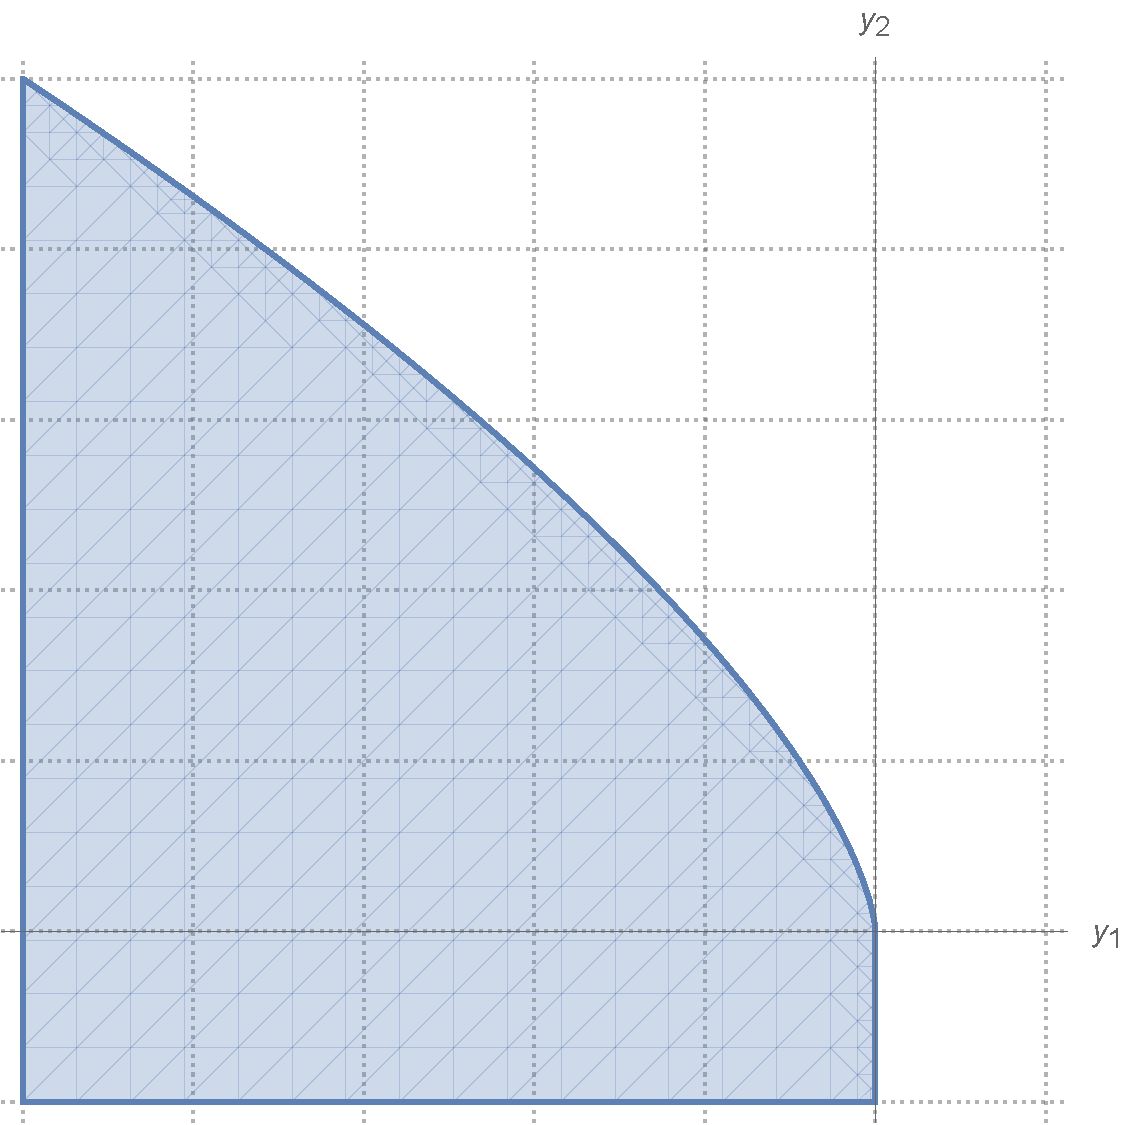
\includegraphics[width=0.6\textwidth]{Problem Set 2 Files/set.pdf}
    \caption{Production Set $Y$}
\end{figure}

\textbf{Part (b)} The firm chooses the amount of $y_1$ and $y_2$ to maximize it's profits:

\begin{align*}
    \max_{y_1,y_2}\quad &\: p_1 y_1 + p_2 y_2\\
     \text{subject to: }\quad &  y_2 \leq B\left(-y_{1}\right)^{\frac{2}{3}}\\
     &y_1\leq 0,\\& y_2\geq 0
\end{align*}

First note that the profits of the firm are increasing in $y_2$ and decreasing in $(-y_1)$, then assume that there is a solution of the maximization problem with 

$$y_2 < B\left(-y_{1}\right)^{\frac{2}{3}}$$

then there are values $\varepsilon, \delta>0$ such that $y_1+\delta \leq 0$ and 

$$y_2 + \varepsilon < B\left(-y_{1}-\delta \right)^{\frac{2}{3}}$$

This means the solution $(y_1+\delta, y_2+\varepsilon)$ is feasible and will yield higher profits to the firm (this is to say the the firm will better off by producing more or using less inputs), this contradicts the assumption that the solution was optimal. Then we can restrict our attention to the set of values for which

$$y_2 = B\left(-y_{1}\right)^{\frac{2}{3}}$$

This gives the following maximization problem in one variable

$$\max_{y_1}\quad &\: p_1 y_1 + p_2 B\left(-y_{1}\right)^{\frac{2}{3}} $$

This problem have a first order condition:

\begin{align*}
p_1-\frac{2 B p_2}{3 \sqrt[3]{-y_1}} = 0 &\qiq y_1 = -\left(\frac{2 B p_2}{3 p_1}\right)^3\\
&\qiq y_2 = \frac{4 B^3 p_2^2}{9 p_1^2}    
\end{align*}

Then:

$$Y^*(p)=\left(-\left(\frac{2 B p_2}{3 p_1}\right)^3, \frac{4 B^3 p_2^2}{9 p_1^2}     \right) \qquad  \pi(p) = \frac{4 B^3 p_2^3}{27 p_1^2}$$

\textbf{Part (c)}

To show that $\pi(p)$ is homogeneous of degree $1$ consider

$$\pi(\alpha p) = \frac{4 B^3 \alpha^3 p_2^3}{27 \alpha^2 p_1^2} = \alpha \frac{4 B^3 p_2^3}{27 p_1^2} = \alpha^1 \pi(p)$$

Next we show that $y(p)$ is homogeneous of degree $0$,

\begin{align*}
y(\alpha p) &=  \left(\left(\frac{2 B \cancel{\alpha} p_2}{3 \cancel{\alpha} p_1}\right)^3, \frac{4 B^3 \cancel{\alpha^2} p_2^2}{9 \cancel{\alpha}^2 p_1^2} \right)= y(p) = \alpha^0 y(p)
\end{align*}

\textbf{Part (d)}
We check Hotelling's lemma

$$\frac{\partial \pi}{\partial p_1} (p) = -\frac{8 B^3 p_2^3}{27 p_1^3} = y_1(p)$$

$$\frac{\partial \pi}{\partial p_2} (p) = \frac{4 B^3 p_2^2}{9 p_1^2} = y_2(p)$$

\textbf{Part (e)}

We know that:

$$D_p y(p) = \left(\begin{array}{cc}
\partial y_1/\partial p_1     &  \partial y_1/\partial p_2  \\
\partial y_2/\partial p_1 & \partial y_2/\partial p_2
\end{array}\right)$$


Calculating the derivatives we get

$$D_p y(p) = \left(\begin{array}{cc}
\frac{8 B^3p_1^3}{9p_1^4}     &  -\frac{8 B^3p_2^2}{9p_1^3}\\
-\frac{8 B^3p_2^2}{9p_1^3}     &  \frac{8 B^3p_2}{9 p_1^2}
\end{array} \right) = \frac{8 B^3p_2}{9p_1^2}\left(\begin{array}{cc}
\frac{p_2^2}{p_1^2}     & -\frac{p_2}{p_1} \\
-\frac{p_2}{p_1}     & 1
\end{array} \right) $$

This is clearly a symmetric matrix and since $\frac{8 B^3p_2}{9p_1^2}>0$ we only need to check that:

$$\left(\begin{array}{cc} a & b\end{array} \right)  \left(\begin{array}{cc}
\frac{p_2^2}{p_1^2}     & -\frac{p_2}{p_1} \\
-\frac{p_2}{p_1}     & 1
\end{array} \right) \left(\begin{array}{c} a \\ b \end{array}\right) \geq 0 \qquad \forall  \left(\begin{array}{cc} a & b\end{array} \right) \neq \left(\begin{array}{cc} 0 & 0\end{array} \right)$$

After multiplying the matrices we obtain

$$a^2 \frac{p_2^2}{p_1^2} - 2ab\frac{p_2}{p_1} + b^2 = \left(a\frac{p_2}{p_1}-b\right)^2\geq 0$$

Therefore $D_p y(p)$ is positive semidefinite.

$$D_p y(p) = \frac{8 B^3p_2}{9p_1^2}\left(\begin{array}{cc}
\frac{p_2^2}{p_1^2}     & -\frac{p_2}{p_1} \\
-\frac{p_2}{p_1}     & 1
\end{array} \right)}\left(\begin{array}{cc}
p_1 \\
p_2
\end{array} \right)  =  \frac{8 B^3}{9}\left(\begin{array}{l}
\frac{p_{2}^{3}}{p_{1}^{3}}-\frac{p_{2}^{3}}{p_{1}^{3}} \\
-\frac{p_{2}^{2}}{p_{1}^{2}}+\frac{p_{2}^{2}}{p_{1}^{2}}
\end{array}\right) = \left(\begin{array}{cc}0\\0\end{array}\right)$$

\end{proof}

\begin{problem}[\textbf{...and recovering technology from the profit function}]
Finally, suppose we didn't know a firm's production set $Y$, but did know its profit function was
$$
\bar{\pi}(p)=A p_{1}^{-2} p_{2}^{3}
$$
for all $p_{1}, p_{2}>0$ and $A>0$ a known constant.
\begin{enumerate}[(a)]
    \item What conditions must hold for this profit function to be rationalizable? (You don't need to check them.)
    \item Recall that the outer bound was defined as
        $$
        Y^{O}=\{y \quad: \quad p \cdot y \quad \leq \quad \pi(p) \quad \text { for all } \quad p \in P\}
        $$
        In this case, this is
        $$
        Y^{O}=\left\{\left(y_{1}, y_{2}\right): \quad p_{1} y_{1}+p_{2} y_{2} \leq A p_{1}^{-2} p_{2}^{3} \quad \text { for all } \quad\left(p_{1}, p_{2}\right) \in \mathbb{R}_{++}^{2}\right\}
    $$
    Show that any $y \in Y^{O}$ must have $y_{1} \leq 0,$ i.e., that good 1 must be an input only.
    \item Dividing both sides by $p_{2}$ and moving $\frac{p_{1}}{p_{2}} y_{1}$ to the right-hand side, we can rewrite $Y^{O}$ as
    $$
    Y^{O}=\left\{\left(y_{1}, y_{2}\right): \quad y_{2} \leq A p_{1}^{-2} p_{2}^{2}-\frac{p_{1}}{p_{2}} y_{1} \quad \text { for all } \quad\left(p_{1}, p_{2}\right) \in \mathbb{R}_{++}^{2}\right\}
    $$
    since the expression on the right depends only on the price ratio $\frac{p_{2}}{p_{1}}$ rather than the two individual prices, we can let $r \equiv \frac{p_{2}}{p_{1}}>0$ denote this ratio, and write $Y^{O}$ as
    $$
    \begin{aligned}
    Y^{O} &=\left\{\left(y_{1}, y_{2}\right): y_{2} \leq A r^{2}-\frac{y_{1}}{r} \quad \text { for all } r \in \mathbb{R}_{++}\right\} \\
    &=\left\{\left(y_{1}, y_{2}\right): y_{2} \leq \min _{r>0}\left(A r^{2}-\frac{y_{1}}{r}\right)\right\}
    \end{aligned}
    $$
    Solve this minimization problem, and describe the production set $Y^{O}$.
    \item  Verify that a production set $Y$ equal to the set $Y^{O}$ you just calculated would generate the "data" $\pi(p)=A p_{1}^{-2} p_{2}^{3}$ that we started with.
    
    If you feel you've already done enough algebra on this assignment, you may use the fact that $\left(2^{-2 / 3}+2^{1 / 3}\right)^{3}=\frac{27}{4}$ without calculating it.
    
    If you already did question $2,$ you can use what you found there, and this question should not take you very long.
    \end{enumerate}
\end{problem}

\begin{proof}[Answer]
\textbf{Part (a)} $\pi(p)$ have to be homogeneous of degree 1 and convex.
\newline
\newline
\textbf{Part (b)} For any price vector for any $y_1>0$ we can take a price vector with $p_1$ sufficiently large so that $p_{1} y_{1}+p_{2} y_{2} > A p_{1}^{-2} p_{2}^{3}$. then if we assume that there is an element of $Y^O$ with $y_1$ negative we can "prove" that that that element is not in $Y^O$ thus contradicting our initial assumption.
\newline
\newline
\textbf{Part (c)} The function 

$$A r^{2}-\frac{y_{1}}{r}$$

have a first order condition:

$$2 A r+\frac{y_1}{r^2} = 0 \qiq r^* &=\Big( \frac{-y_1}{2A}\Big)^\frac{1}{3} $$

the second order condition 

$$2 A-\frac{2 y_1}{r^3}>0$$

Tells us this is in fact a global minimum since the function is convex.

Plugging in the objective function, we get 
$$A \Big(\frac{-y_1}{2A}\Big)^{\frac{2}{3}} - y_1 \Big(\frac{-y_1}{2A}\Big)^{\frac{1}{3}} = (2^\frac{1}{3}+ 2^\frac{-2}{3}) A^\frac{1}{3}(-y_1)^{\frac{2}{3}}$$
Then:
$$ Y^O = \Big\{(y_1,y_2) : y_1 \leq 0 \text{ and } y_2 \leq  (2^\frac{1}{3}+ 2^\frac{-2}{3}) A^\frac{1}{3}(-y_1)^{\frac{2}{3}}\Big \} $$

\textbf{Part (d)} Make $B = (2^\frac{1}{3}+ 2^\frac{-2}{3}) A^\frac{1}{3}$ and if we plug in this expression in to the profits function that we obtained from \textbf{Problem 2} we get:

 $$\pi(p) = \frac{4 B^3 p_2^3}{27 p_1^2} = \frac{4 \Big(  (2^\frac{1}{3}+ 2^\frac{-2}{3}\Big ) A^\frac{1}{3})^3 p_2^3}{27 p_1^2} = \frac{A p_2^3}{p_1^2} $$



\end{proof}

\end{document}
